% =====================================================================
% AI Academy -- National AI Center
% Software Engineering Final Project -- Final Report
%
% Topic 4 -- Async Research Assistant
% Produced from templates/REPORT_TEMPLATE.tex.
%
% Compile with pdfLaTeX (two passes, for LastPage and the table of
% contents):  pdflatex report.tex && pdflatex report.tex
% =====================================================================

\documentclass[10pt,a4paper]{article}

% ===== EARLY MACROS (must come before configuration) =================
\usepackage[dvipsnames]{xcolor}
\definecolor{accent2}{HTML}{8B0000}
\definecolor{ph}{HTML}{6B7280}
\newcommand{\TODO}[1]{\textcolor{accent2}{\textbf{[TODO: #1]}}}
\newcommand{\phh}[1]{\textcolor{ph}{\textit{#1}}}

% ===== CONFIGURATION =================================================
% No official team name; members are listed by GitHub handle.
\newcommand{\teamname}{}
\newcommand{\topicchoice}{Topic 4 --- Async Research Assistant}
\newcommand{\member}[2]{\textbf{#1} (#2)}  % name, GitHub handle
\newcommand{\reportdate}{2026-09-19}
\newcommand{\repolink}{\url{https://github.com/ii1ahe/research-assistant}}

% ===== course meta (rarely changes) ==================================
\newcommand{\coursecode}{AI-ENG-110}
\newcommand{\coursename}{Software Engineering}
\newcommand{\institution}{AI Academy, National AI Center}
\newcommand{\semester}{Spring 2026}

% ===== PACKAGES ======================================================
\usepackage[margin=2cm,headheight=15pt]{geometry}
\usepackage[T1]{fontenc}
\usepackage[utf8]{inputenc}
\usepackage[final,protrusion=true,expansion=false]{microtype}
\usepackage{amsmath,amssymb}
\usepackage{graphicx}
\usepackage{booktabs}
\usepackage{array}
\usepackage{tabularx}
\usepackage{ragged2e}
\usepackage{enumitem}
\usepackage[parfill]{parskip}
\setlength{\parskip}{1.5pt}
\usepackage{listings}
\usepackage[most]{tcolorbox}
\usepackage{titlesec}
\usepackage{fancyhdr}
\usepackage{lastpage}
\usepackage{etoolbox}
\usepackage{tikz}
\usetikzlibrary{arrows.meta,positioning,fit,backgrounds}
\usepackage[hidelinks]{hyperref}

\emergencystretch=3em
\hbadness=10000
\hfuzz=2pt
\linespread{0.96}

\hypersetup{
  colorlinks=true,
  linkcolor=NavyBlue,
  urlcolor=NavyBlue,
  citecolor=NavyBlue,
  pdftitle={\coursecode\ Final Project Report},
  pdfauthor={Async Research Assistant}
}

% ===== STYLING =======================================================
\definecolor{accent}{HTML}{0B3D91}
\definecolor{soft}{HTML}{F2F4F8}
\definecolor{deliver}{HTML}{E8F0FE}
\definecolor{deliverframe}{HTML}{1A56DB}
\definecolor{probe}{HTML}{FFF8E1}
\definecolor{probeframe}{HTML}{B45309}

\titleformat{\section}
  {\Large\bfseries\color{accent}}{\thesection.}{0.6em}{}
\titleformat{\subsection}
  {\large\bfseries\color{accent}}{\thesubsection}{0.5em}{}
% Tighter vertical rhythm than the template default: the report runs long and
% the template's own target is 8-10 pages.
\titlespacing*{\section}{0pt}{1.05ex plus .2ex minus .1ex}{0.6ex}
\titlespacing*{\subsection}{0pt}{0.8ex plus .1ex minus .05ex}{0.4ex}

\newcommand{\ans}[1]{\rule[-2pt]{#1}{0.5pt}}
\let\ph\phh

% A light callout reused for the two findings worth pulling out of the prose.
\newtcolorbox{findingbox}{
  colback=deliver, colframe=deliverframe, boxrule=0.5pt,
  arc=2pt, left=8pt, right=8pt, top=4pt, bottom=4pt
}

\definecolor{codegreen}{rgb}{0,0.55,0}
\definecolor{codegray}{rgb}{0.4,0.4,0.4}
\definecolor{codepurple}{rgb}{0.55,0,0.78}
\definecolor{backcolour}{rgb}{0.97,0.97,0.97}

\lstdefinestyle{python}{
  language=Python,
  backgroundcolor=\color{backcolour},
  commentstyle=\color{codegreen},
  keywordstyle=\color{accent},
  numberstyle=\tiny\color{codegray},
  stringstyle=\color{codepurple},
  basicstyle=\ttfamily\footnotesize,
  breakatwhitespace=false,
  breaklines=true,
  keepspaces=true,
  numbers=left,
  numbersep=6pt,
  tabsize=2,
  frame=single,
  framerule=0.4pt,
  rulecolor=\color{black!30},
}

\pagestyle{fancy}
\fancyhf{}
\fancyhead[L]{\small\textit{\coursecode\ -- Final Report\ifdefempty{\teamname}{}{\ -- \teamname}}}
\fancyhead[R]{\small\textit{\semester}}
\fancyfoot[L]{\small\textit{\institution}}
\fancyfoot[R]{\small Page \thepage\ of \pageref{LastPage}}
\renewcommand{\headrulewidth}{0.4pt}
\renewcommand{\footrulewidth}{0.4pt}

% =====================================================================
\begin{document}

\begin{center}
{\small \textsc{\institution} \\[0.2em] \textsc{\coursecode\ -- \coursename\ -- \semester}}\\[1.2em]
{\Large\bfseries\color{accent} Final Project Report}\\[0.3em]
{\LARGE\bfseries \topicchoice}\\[0.6em]
\rule{0.85\textwidth}{0.6pt}
\end{center}

\vspace{0.6em}
\begin{tabularx}{\textwidth}{@{}lXlX@{}}
\textbf{Team:} & No official name & \textbf{Date:} & \reportdate \\
\textbf{Repo:} & \repolink & \textbf{Tag:} & \texttt{v1.0-final} \\
\textbf{Members:} & \multicolumn{3}{X@{}}{%
  \texttt{@ii1ahe} \quad \texttt{@fatimekazimli} \quad \texttt{@Elmin995}
}\\
\end{tabularx}
\vspace{0.3em}\hrule\vspace{0.4em}

% ===== EXECUTIVE SUMMARY =============================================
\section*{Executive Summary}
\addcontentsline{toc}{section}{Executive Summary}

We built \textbf{Researcher}, a command-line research assistant that takes one natural-language
question, retrieves evidence from Wikipedia, arXiv and the open web \emph{concurrently}, and
returns a single answer with numbered citations pointing back at the sources it actually used.
Each source fetch has its own deadline, so a slow or dead source costs one
citation rather than the whole run; the answer is synthesised once through the supplied AI module,
validated structurally, and stored in PostgreSQL with a cache of retrieval results.
The headline concurrency number is \textbf{1.67$\times$}: retrieval for five questions fell from
4.83\,s to 2.89\,s with three sources in flight --- 92\,\% of the 1.83$\times$ ceiling the
slowest single source imposes.
The headline robustness story is that \emph{partial results are a first-class outcome, not an
error}: a run that loses one source still answers, and says which one, because exit~0 with a
disclosed gap is more useful to a researcher than a clean failure.
The most surprising finding is that end-to-end speedup is \textbf{1.00$\times$} --- retrieval is
11\,\% of wall-clock time and the synthesis call that follows is the other 89\,\%, so a phase of
concurrency work is invisible to the user until the model call shrinks too.
A second surprise came from the benchmark itself: our first attempt reported 4.65$\times$ by
comparing real work against fast failures, which is why it now withholds a row unless every
question in both sweeps was answered.
If we started over, we would build the benchmark in Phase~2 --- every defect worth reporting here
was found by measuring, not by reading.

% ===== TABLE OF CONTENTS =============================================
\setcounter{tocdepth}{1}
\vspace{0.2em}
\tableofcontents
\vspace{0.3em}\hrule\vspace{0.3em}

% =====================================================================
\section{Project Overview}

\subsection{Problem framing and scope}

A researcher asking a question of the open web faces three chores that are mechanical, slow, and
easy to get wrong: deciding \emph{where} to look, issuing those lookups without waiting for each
one in turn, and keeping track of which claim came from which page. Researcher automates all
three and is deliberately narrow about it. It answers \emph{one} question per invocation, from
\emph{three} named source families, and it never presents a claim it cannot attach to a numbered
source.

The scope boundary is set by what the system refuses to do. It has \textbf{no HTTP API} (ADR-006)
--- the deliverable is a CLI program and the container publishes no port; an API would add an
authentication surface, concurrency semantics and a lifecycle this topic does not ask for. It
makes \textbf{no answer-quality claim}: it verifies that an answer is \emph{internally
consistent}, never that its sources
support its claims (Section~\ref{sec:limits}). And it offers \textbf{no second opinion} --- one
provider, one model --- an ensemble would triple the quota cost of a demo run, the binding
constraint on a free tier (Section~\ref{sec:politeness}).

The inputs are a question, a set of source names and a results-per-source limit; the output is a
rendered answer, a numbered source list, a per-source retrieval report, and a process exit status
(Table~\ref{tab:exitcodes}). The last is load-bearing: the program distinguishes ``answered'' from
``answered but incomplete'' from ``no usable answer'' from ``you invoked it wrong'', because a
script wrapping this tool needs that distinction and a single non-zero code would erase it.

\begin{table}[htbp]
\centering
\footnotesize
\caption{Exit statuses. Zero is returned for a disclosed partial answer, because a run that loses
one source has still done useful work.}
\label{tab:exitcodes}
\begin{tabularx}{\textwidth}{@{}clX@{}}
\toprule
\textbf{Code} & \textbf{Name} & \textbf{Meaning} \\
\midrule
0 & \texttt{EXIT\_OK} & Answered. May carry warnings naming failed sources; those are printed. \\
1 & \texttt{EXIT\_FAILURE} & No usable answer, or a required persistence write failed. \\
2 & \texttt{EXIT\_USAGE} & Invalid input or configuration, detected before any I/O. \\
\bottomrule
\end{tabularx}
\end{table}

\subsection{Provider choice and the AI module contract}

The supplied \texttt{ai/} package is a fixed contract (TOPIC.md, lines 90--94) and is imported
and never modified, so the project's job is to \emph{use} it well rather than to extend it. It
supplies two things: source fetchers (\texttt{fetch\_wikipedia}, \texttt{fetch\_arxiv},
\texttt{fetch\_web}) returning a list of \texttt{Source} records, and \texttt{synthesize}, which
takes a question and a list of sources and returns an \texttt{AnswerWithCitations}.

We run on \textbf{Gemini} via the supplied \texttt{GeminiLLM} provider on
\texttt{gemini-3.1-flash-lite}, with Tavily for web search and key-free Wikipedia and arXiv for the
rest. Two facts about that choice are worth recording. First, the providers in
\texttt{ai/providers/google.py} fall back to \texttt{gemini-2.0-flash}, which is retired --- every
2.x model returns HTTP~404, so the application configures the model explicitly rather than relying
on the supplied default. Second, Gemini's 3.x models emit \emph{reasoning} tokens that count
against the same \texttt{max\_output\_tokens} budget as the answer, so the synthesis budget must
leave room for the reasoning before the answer begins.

\paragraph{One documented divergence.} The supplied \texttt{ai.sources.fetch\_wikipedia} cannot
answer a natural-language question. It searches with the MediaWiki \texttt{opensearch} API, which
prefix-matches the \emph{entire} query against article \emph{titles}. Measured:

\begin{center}
\footnotesize
\begin{tabular}{@{}llr@{}}
\toprule
\textbf{Query sent} & \textbf{Matching mode} & \textbf{Titles returned} \\
\midrule
\texttt{What is photosynthesis and what are its main stages?} & prefix match & 0 \\
\texttt{photosynthesis} & prefix match & 3 \\
\texttt{photosynthesis main stages} & prefix match & 0 \\
\bottomrule
\end{tabular}
\end{center}

Multi-word queries match nothing, so no query-rewriting heuristic recovers this --- keyword
derivation was our first idea and fails too, because \texttt{photosynthesis main stages} already
is the derivation. Since \texttt{ai/} is
immutable, \texttt{researcher/services/wikipedia.py} replaces the \emph{search step only},
using the MediaWiki \texttt{list=search} full-text endpoint, and keeps the supplied summary
endpoint and the supplied \texttt{Source} shape. The setting
\texttt{WIKIPEDIA\_SEARCH=fulltext|opensearch} selects between them and defaults to
\texttt{fulltext}, so the supplied path stays reachable and testable rather than being deleted.
This divergence is the single place where our behaviour differs from the supplied module, and it
is deliberate, documented in the module docstring, and reversible by configuration.

% =====================================================================
\section{Architecture}

\subsection{Module map}

The system is a layered modular monolith with a flat package layout: \texttt{ai/} and
\texttt{researcher/} sit side by side at the repository root. ADR-001 records why ---
\texttt{ai/} must be importable as a top-level package because the contract fixes it there, and a
flat layout means the stock \texttt{python:3.14.7-slim} image works with a plain
\texttt{COPY} and a \texttt{WORKDIR}, with no \texttt{pip install .} and no packaging step. The application is 4\,681 lines across 25 source files; the layering rule is enforced
by import direction rather than by tooling, so a lower layer never imports from a higher one.

\begin{figure}[htbp]
\centering
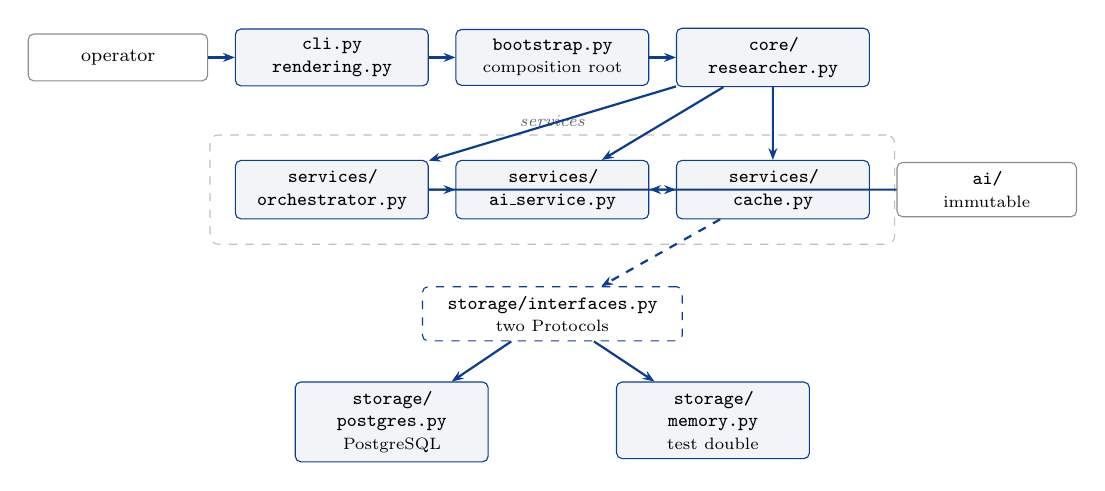
\begin{tikzpicture}[
  scale=0.85, transform shape,
  font=\footnotesize,
  box/.style={draw=accent, rounded corners=2pt, fill=soft, align=center,
              inner sep=4pt, minimum height=7mm, text width=26mm},
  iface/.style={draw=accent, dashed, rounded corners=2pt, fill=white, align=center,
                inner sep=4pt, minimum height=7mm, text width=36mm},
  ext/.style={draw=black!45, rounded corners=2pt, fill=white, align=center,
              inner sep=4pt, minimum height=7mm, text width=24mm},
  arrow/.style={-{Stealth[length=1.5mm]}, draw=accent, thick},
  note/.style={font=\scriptsize\itshape, text=black!60, align=center}
]

% Row 1 -- presentation and composition
\node[ext] (user) {operator};
\node[box, right=4mm of user] (cli) {\texttt{cli.py}\\\texttt{rendering.py}};
\node[box, right=4mm of cli] (boot) {\texttt{bootstrap.py}\\{\scriptsize composition root}};
\node[box, right=4mm of boot] (core) {\texttt{core/}\\\texttt{researcher.py}};

% Row 2 -- the services layer
\node[box, below=11mm of cli] (orch) {\texttt{services/}\\\texttt{orchestrator.py}};
\node[box, right=4mm of orch] (aisvc) {\texttt{services/}\\\texttt{ai\_service.py}};
\node[box, right=4mm of aisvc] (cache) {\texttt{services/}\\\texttt{cache.py}};
\node[ext, right=4mm of cache] (ai) {\texttt{ai/}\\{\scriptsize immutable}};

% Row 3 -- the storage seam
\node[iface, below=10mm of aisvc] (store) {\texttt{storage/interfaces.py}\\{\scriptsize two Protocols}};

% Row 4 -- the two implementations
\node[box, below=6mm of store, xshift=-24mm] (pg) {\texttt{storage/}\\\texttt{postgres.py}\\{\scriptsize PostgreSQL}};
\node[box, below=6mm of store, xshift=24mm] (mem) {\texttt{storage/}\\\texttt{memory.py}\\{\scriptsize test double}};

\draw[arrow] (user) -- (cli);
\draw[arrow] (cli) -- (boot);
\draw[arrow] (boot) -- (core);
\draw[arrow] (core) -- (orch);
\draw[arrow] (core) -- (aisvc);
\draw[arrow] (core) -- (cache);
\draw[arrow] (orch) -- (aisvc);
\draw[arrow] (orch) -- (cache);
\draw[arrow] (ai) -- (aisvc);
\draw[arrow, dashed] (cache) -- (store);
\draw[arrow] (store) -- (pg);
\draw[arrow] (store) -- (mem);

\begin{scope}[on background layer]
\node[draw=black!25, dashed, rounded corners=3pt, inner sep=9pt,
      fit=(orch)(aisvc)(cache), label={[note]above:services}] {};
\end{scope}

\end{tikzpicture}
\caption{Module map. Solid arrows are ordinary calls; the dashed arrow into
\texttt{storage/interfaces.py} is the seam where behaviour is substituted in tests. The two
implementations under that seam are interchangeable because the interface is a \texttt{Protocol},
not a base class (Section~\ref{sec:oop}).}
\label{fig:modules}
\end{figure}

\begin{table}[htbp]
\centering
\footnotesize
\caption{The modules that carry the design, and the single responsibility each owns.}
\label{tab:modules}
\begin{tabularx}{\textwidth}{@{}lrX@{}}
\toprule
\textbf{Module} & \textbf{LOC} & \textbf{Responsibility} \\
\midrule
\texttt{models.py} & 371 & The frozen Pydantic models every layer exchanges. \\
\texttt{validation.py} & 390 & Normalising input; validating a synthesised answer. \\
\texttt{config.py} & 316 & Typed settings, derived flags, safe error messages. \\
\texttt{errors.py} & 181 & The exception taxonomy and the exit-status mapping. \\
\texttt{services/orchestrator.py} & 249 & Bounded concurrent retrieval; one outcome per source. \\
\texttt{services/ai\_service.py} & 599 & The only place \texttt{ai/} is called; timeouts, retries, translation. \\
\texttt{services/cache.py} & 199 & Cache-aside reads and writes around the storage seam. \\
\texttt{services/resilience.py} & 233 & The retry policy and its backoff schedule. \\
\texttt{storage/interfaces.py} & 146 & The two \texttt{Protocol}s and the error contract. \\
\texttt{storage/postgres.py} & 293 & \texttt{asyncpg} implementation; migrations applied at startup. \\
\texttt{storage/memory.py} & 125 & In-memory double; the fast test tier runs against it. \\
\texttt{core/researcher.py} & 256 & The use case: retrieve, synthesise, validate, persist. \\
\texttt{bootstrap.py} & 284 & The composition root --- the only module naming concrete classes. \\
\texttt{cli.py}, \texttt{rendering.py} & 584 & Argument parsing, exit statuses, terminal rendering. \\
\bottomrule
\end{tabularx}
\end{table}

\subsection{OOP design and key abstractions}
\label{sec:oop}

Three decisions carry most of the design.

\paragraph{Structural typing at the seams, inheritance nowhere.} The two storage seams ---
\texttt{SourceCacheStore} and \texttt{SessionRepository} --- are \texttt{typing.Protocol}
classes, and the code depends on the protocol rather than on a concrete implementation. Protocols beat
abstract base classes for a testability reason: an
\texttt{ABC} imposes a nominal relationship, so a test double either inherits from the real
implementation or the type checker objects. A \texttt{Protocol} is satisfied structurally, which
means \texttt{storage/memory.py} is a genuine second implementation that the production code
cannot distinguish from \texttt{storage/postgres.py}, and \texttt{tests/test\_storage.py} runs
the \emph{same} contract suite against both. That is the difference between a mock that agrees
with the code and an implementation that agrees with the interface.

\paragraph{Frozen models at every boundary.} Every value crossing a layer is a frozen Pydantic
model with \texttt{extra="forbid"} --- \texttt{ResearchRequest}, \texttt{Source},
\texttt{SourceOutcome}, \texttt{RetrievalResult}, \texttt{ResearchResult},
\texttt{ResearchSession}. There are no naked dictionaries in the application's own interfaces.
Frozen models give immutability for free, and \texttt{extra="forbid"} makes a typo in a
keyword argument an error at construction rather than a silently ignored field --- valuable in a
system whose failure modes are mostly ``a source quietly returned nothing''. One deliberate exception is \texttt{AnswerWithCitations}, which is the supplied module's
type and is therefore validated but not replaced.

\paragraph{One composition root.} \texttt{bootstrap.py} is the only module that names a concrete
class. Everything else receives its collaborators as constructor arguments, which is what makes
the fast test tier possible: the orchestrator tests construct an orchestrator with an in-memory
cache and a fake AI service, with no database, no network, and no API key. The dependency graph
is assembled once, in one readable place, rather than resolved at each use site.

Two smaller abstractions earn their keep. \texttt{RetryPolicy} in
\texttt{services/resilience.py} separates \emph{whether} to retry from \emph{what} is being
retried, so the same policy covers HTTP fetches and model calls with different settings
(\texttt{max\_attempts}=3, exponential backoff from 0.5\,s capped at 8\,s, full jitter). And
\texttt{SourceOutcome} models a per-source retrieval as a value carrying either the sources or
the reason it failed, so ``source X is unavailable'' becomes data the renderer prints rather than
an exception that unwinds the run.

\subsection{Data flow: one question, end to end}

A request enters at \texttt{cli.py}, which parses and validates before any I/O: an unknown source
name, an empty or over-long question, or a missing credential for the selected provider is
rejected here with exit~2. \texttt{bootstrap.py} then builds the
object graph --- settings, a shared \texttt{httpx} client, the AI service, the cache over a
PostgreSQL store, and the session repository --- and \texttt{ResearchService.research} asks the
orchestrator for sources. The orchestrator canonicalises the query once, so two questions
differing only in whitespace share a cache entry, then consults the cache per source: a hit
returns the stored records with \texttt{attempts=0}, a miss acquires a slot on an
\texttt{asyncio.Semaphore} and calls the AI service under \texttt{per\_source\_timeout\_seconds}.

The AI service is the only module that touches \texttt{ai/} --- it classifies the provider's
failure, decides whether the retry policy should see it, and translates it into our own
\texttt{UpstreamError}. \texttt{gather(..., return\_exceptions=True)} rejoins the tasks and every
result, success or failure, becomes a \texttt{SourceOutcome}; a \texttt{CancelledError} is
re-raised rather than converted, because swallowing it would break task cancellation. If no
source produced anything the run stops with exit~1. Otherwise the AI service synthesises once
under its own deadline, and \texttt{validate\_answer} checks every citation index against the
source list actually sent --- positive, unique, in range, and not reordered after synthesis,
which would silently repoint every reference number in the prose. The session is persisted as one
JSON document, and the renderer prints the answer, the numbered sources and the per-source
report.

% =====================================================================
\section{Concurrency \& Performance}

\subsection{Why this model}

The work per question is a fan-out with no dependencies: three sources, each an independent
network round trip, none needing another's output. That is the ideal shape for \texttt{asyncio}
--- I/O-bound, data-independent tasks, where threads would add preemption and locking for no
benefit. The whole application is single-threaded.

Two design points matter more than the choice of library. First, \textbf{the bound is a
\texttt{Semaphore}, not a bigger gather.} Every source task acquires a slot on
\texttt{asyncio.Semaphore(max\_parallel\_sources)}, default three. Three sources and a bound of
three make that look redundant, and it is not: the bound is what keeps a request with six
sources from opening six simultaneous connections to Wikipedia, and it is the knob an operator
turns when a provider starts complaining --- a configuration change either way, because the
limit is not the size of the \texttt{gather}. Second, \textbf{there is no timeout wrapping the
\texttt{gather}, deliberately.} A deadline around the group would let one slow source destroy
the results of two fast ones that had already arrived; instead each task is bounded
individually, so nothing that succeeded is thrown away. Total latency is therefore bounded by
the per-source timeout rather than by the sum, which is the right trade for a system whose
output is a citation list.

\subsection{Sequential vs concurrent benchmark}

\texttt{scripts/bench.py} drives the assembled application twice over the same five supplied
sample questions, once with \texttt{max\_parallel\_sources=1} and once with the default 3, and
writes \texttt{artefacts/bench.json} and a human-readable report. It measures retrieval alone and
the full end-to-end path.

\begin{table}[htbp]
\centering
\footnotesize
\caption{Measured against live Wikipedia, arXiv, Tavily and Gemini, five sample questions,
\texttt{max\_results\_per\_source}=3. Retrieved 2026-09-16; raw output in
\texttt{artefacts/bench.json}.}
\label{tab:bench}
\begin{tabular}{@{}lrrr@{}}
\toprule
\textbf{Workload} & \textbf{Sequential} & \textbf{Concurrent} & \textbf{Speedup} \\
 & (bound 1) & (bound 3) & \\
\midrule
Retrieval, 5 questions $\times$ 3 sources & 4.83\,s & 2.89\,s & \textbf{1.67$\times$} \\
Retrieval, per question (mean)            & 0.97\,s & 0.58\,s & \textbf{1.67$\times$} \\
End-to-end, 5 questions                   & 43.4\,s & 43.3\,s & \textbf{1.00$\times$} \\
\midrule
\multicolumn{3}{@{}l}{Ceiling for three sources, $\sum t_i / \max t_i$} & 1.83$\times$ \\
\bottomrule
\end{tabular}
\end{table}

The retrieval figure needs its ceiling stated, because 1.67$\times$ looks disappointing against
the naive expectation of 3$\times$ and is not. With three independent tasks of latency
$t_1, t_2, t_3$, sequential execution takes $\sum t_i$ and concurrent execution takes
$\max t_i$, so the best any schedule can achieve is $\sum t_i / \max t_i$ --- which depends
entirely on how uneven the sources are. For this source mix the ceiling is 1.83$\times$, so the
measured 1.67$\times$ is \textbf{92\,\% of the achievable maximum}; the gap is scheduling
overhead and the cache lookups preceding each fetch. A more even mix would show a larger ratio and a mix with one dominant source almost none ---
which is why the ceiling is reported beside the number.

The end-to-end row is the finding that matters, and it is the opposite of flattering. Retrieval
was 4.83\,s of a 43.4\,s run --- about 11\,\% --- and the rest is synthesis, one sequential model
call per question, untouched by the concurrency design. The honest summary of an entire phase of
work is that \textbf{it optimised 11\,\% of the runtime}. The design is correct and the
measurement is real; the number is simply small, and saying so is more useful than reporting
only the row that flatters.

\begin{findingbox}
\textbf{The first version of this benchmark lied to us.} It reported a \textbf{4.65$\times$}
end-to-end speedup. The cause was not a measurement bug but a comparison bug: when Gemini's free
tier refused a synthesis, the call returned in roughly a second instead of eight, so the
sequential sweep was being timed against real work while the concurrent sweep was partly timed
against fast failures. The script now \emph{withholds} the synthesis and end-to-end rows unless
every question in \emph{both} sweeps was actually answered, prints the reason, and exits~1 --- so
a run that cannot produce a fair comparison produces no comparison rather than a wrong one. This
is the single most useful thing we built, because it found the next defect too.
\end{findingbox}

\subsection{Rate limits and politeness}
\label{sec:politeness}

\texttt{MAX\_PARALLEL\_SOURCES} bounds how many of \emph{our} tasks are in flight. It is a
politeness limit on our own behaviour and it is not a rate limit: it does not know what the
provider's quota is. What it does now, since the measurement below, is react to being throttled
--- the provider's own retry instruction is honoured instead of ignored.

The free tier for the configured model permits \textbf{20 generation requests per day, per
model}, and a demo run costs five syntheses --- three runs exhaust the bucket. When it ran out,
the provider answered with a payload naming both the limit and the remedy:

\begin{lstlisting}[style=python,numbers=none,caption={The provider's own words, abridged. The
hint is precise, and until the fix below our policy ignored all of it.},captionpos=b]
429 RESOURCE_EXHAUSTED ... limit: 20, model: gemini-3.8-flash
                          Please retry in 21.9s
\end{lstlisting}

Our retry policy then waited a full-jitter backoff of at most 0.5\,s between attempts, so every
attempt landed inside the same throttle window: a throttle the provider described as recoverable
in 22 seconds became a lost question that failed in under a second, with three attempts spent and
a 30-second deadline unused.

Honouring it was not a one-line change, and the reason is a decision we would defend separately:
\texttt{services/ai\_service.py} \emph{deliberately discards} the provider's raw payload when it
translates a failure, so upstream error text can never reach a log or a user. The consequence is
that classification is the last place the \emph{retry hint} exists --- so that is where it is now
parsed: in the exception text first, then in a \texttt{Retry-After} header, since the providers
re-raise with \texttt{from} and the SDK exception's public \texttt{.response.headers} survives
on \texttt{\_\_cause\_\_} --- no SDK import, no private attribute. An HTTP-date rather than
delta-seconds is discarded, because converting one means trusting the local clock against the
server's. A new \texttt{UpstreamRateLimitError} carries the parsed delay (a number,
never the payload text it came from), and the retry policy waits for the larger of its own
jittered backoff and the provider's instruction, uncapped by \texttt{max\_backoff} and bounded
instead by the operation's deadline. A throttle that names no parseable delay is still classified, and still retried on the ordinary
backoff; a test asserts that the measured payload's text never appears in a message.
What remains for production is a token bucket that anticipates a quota instead of discovering
it through the first refused call.

% =====================================================================
\section{Robustness \& Error Handling}

\subsection{Wrapping the AI module}

Everything that can fail in a third-party call is dealt with in \texttt{services/ai\_service.py},
so no other layer has to know what a provider exception looks like.

\paragraph{Failure classification.} The supplied \texttt{ProviderError} is coarse --- a missing
package, a missing credential and a network fault all raise the same type. The service inspects
the message against a set of misconfiguration markers and separates ``this can never succeed''
from ``this might succeed later''. The distinction is not cosmetic: retrying a fault that will
never resolve spends two extra attempts, and giving up on a transient one loses a source.

\paragraph{Translation at the boundary.} Every provider exception becomes an
\texttt{UpstreamError} carrying a safe, generic message and its source. The provider's own text
is dropped on purpose --- a security posture as much as a UX one, since the supplied messages can
quote upstream response text verbatim. Section~\ref{sec:politeness} shows the cost honestly: the
dropped payload is exactly where the retry hint lived.

\paragraph{Timeouts with per-call-type retry semantics.} Fetches are bounded by
\texttt{per\_source\_timeout\_seconds} and \emph{are} retried on timeout, because a search that
has not answered in ten seconds might answer in twelve. Synthesis is bounded separately by
\texttt{synthesis\_timeout\_seconds} and is \emph{not} retried on timeout, because the deadline
wraps the whole call including its retries --- a retried synthesis is guaranteed to hit the same
wall after spending its budget again.

\paragraph{Structural validation of the result.} \texttt{validate\_answer} rejects non-positive,
out-of-range or duplicated citation indices and detects a source list reordered between synthesis
and validation. It also reports the citations the supplied \texttt{synthesize} leaves dangling:
it drops out-of-range indices from the \texttt{citations} list without editing the prose, so the
prose can reference a number that no longer resolves. We surface those rather than rewriting the
model's text.

\subsection{Failure-mode analysis: the throttled synthesis}

The incident worth documenting is the one that reached a user. During the container
verification run, the demo answered three of five questions and the other two came back as
``no usable answer''. The instinctive reading was a packaging fault --- the image was new, the
host was not --- so that is what we tested first, and the test refuted it: the \emph{same}
question, asked from the host against the same database, answered in 2.92\,s. The image was
fine. The provider's daytime quota for that model was spent, and the two failures were the two
questions that arrived after it ran out.

The trace, in the order the layers see it:

\begin{enumerate}[leftmargin=1.6em,itemsep=0.15em]
  \item Gemini returns \texttt{429 RESOURCE\_EXHAUSTED} carrying the limit, the model name and a
        retry hint of 21.9\,s. The provider wrapper raises \texttt{ProviderError} with that
        payload folded into its message.
  \item \texttt{ai\_service} classifies the failure: not a misconfiguration marker, therefore
        retryable. \texttt{RetryPolicy} retries twice more, waiting a jittered $\leq$0.5\,s each
        time, and both attempts land inside the same throttle window.
  \item The attempts are exhausted in under a second. The error becomes an \texttt{UpstreamError}
        with a safe message, and the provider's hint is discarded along with the payload.
  \item The orchestrator converts it into a \texttt{SourceOutcome} carrying a failure reason.
        Synthesis for that question has no sources to work from, so it is reported unanswered.
  \item The run continues: the other three questions answered normally, the CLI printed which
        failed, and the process exited~1 --- the status distinguishing ``some questions failed''
        from ``the program broke''.
\end{enumerate}

What went right is that the failure was contained and legible: one question was lost, not the
run; the user was told which; and the exit status distinguished ``some questions failed'' from
``the program broke''. What went wrong is entirely in steps 3--5: a condition the provider called
recoverable in 22 seconds was treated as unrecoverable in one, because classification asks
whether a failure is the \emph{kind} that can be retried, never \emph{when}.

\subsection{Input validation and exit statuses}

Validation happens in two places, and the split is deliberate. \texttt{validation.py} handles
the \emph{user's} input: source names are normalised and checked against the enumeration,
questions must be non-empty after canonicalisation (a question of pure punctuation is rejected),
the length cap is enforced, and a credential the selected provider requires is checked for at
\emph{startup} rather than at the first call --- so a misconfigured run fails in milliseconds
with a clear message instead of after a timeout with a provider error. Configuration errors
raise \texttt{ConfigurationError} and exit~2.

\texttt{validate\_answer} handles the \emph{model's} output. It rejects an empty or
whitespace-only answer outright: a truncated response or a safety filter would otherwise be
reported as a success, because an answer with no prose tends to have no citations either, and an
empty citation list is vacuously consistent. It then checks citation structure --- every index
positive, in range, unique, and pointing at the source in that position. Content without
citations is still accepted, as a worse answer rather than a missing one. Neither check
establishes that a source supports a claim (Section~\ref{sec:limits}).

% =====================================================================
\section{Storage \& Caching}

\subsection{Schema}

ADR-002 puts \emph{both} persistence concerns --- the retrieval cache and the session store ---
in PostgreSQL, and \texttt{migrations/001\_initial\_schema.sql} is the whole of it. Two tables.

\texttt{source\_cache} stores one row per cached lookup, keyed on the entire cache key --- source,
canonical query, provider, result limit and schema version --- rather than a hash of those
fields. That is deliberate for operability: with the components in separate columns an operator
can \emph{see} what is cached and why a lookup missed, which a digest column would hide. The
write path is \texttt{INSERT \ldots ON CONFLICT} against exactly that key, so the upsert is
enforced by the database rather than by a read-then-write. Three \texttt{CHECK} constraints
mirror the model's numeric bounds, and \texttt{expires\_at >= fetched\_at} is checked because a
row that expires before it was fetched is a bug in the writer, not a user-visible state.

\texttt{research\_sessions} stores the session as one JSON document holding the whole model,
including the per-source outcomes and snippets --- the supplied
\texttt{AnswerWithCitations.to\_dict()} is a presentation format that drops them, so it is not an
archival record. Three columns are denormalised out of the payload so that listing recent
sessions can order and page without parsing every document, and they are deliberately \emph{not}
constrained to the Python enumeration whose values they hold: duplicating a Python enum as a SQL
\texttt{CHECK} would mean a new status could only be added by shipping a migration. The payload
is validated against the model on read, so a bad value surfaces as a \texttt{StorageError}
rather than as a wrong answer.

Migrations are discovered from the filesystem, recorded by filename with a checksum verified on
every later start, so they are append-only: editing an already-applied file is refused rather
than silently skipped, and every statement is idempotent, so a partially applied migration can be
re-run safely. The schema is applied automatically at
startup, which is why \texttt{migrations/} had to be in the container image
(Section~\ref{sec:docker}).

\subsection{Caching policy}

The cache is a cache-aside read in front of every source fetch. The policy is:

\begin{itemize}[leftmargin=1.4em,itemsep=0.15em]
  \item \textbf{Keyed on the canonical query}, not the raw one --- two questions differing only
        in case or whitespace share an entry, which makes a re-run cheap. It strips edge
        punctuation only, never a character \emph{inside} a word, so \texttt{C} and \texttt{C\#}
        are separate keys: over-normalising costs a silent wrong \emph{hit}, under-normalising
        only a \emph{miss}.
  \item \textbf{TTL of \texttt{cache\_ttl\_seconds}} (default 86\,400\,s, one day), stored as an
        absolute \texttt{expires\_at} rather than an age, so expiry does not depend on any
        clock agreeing about when the row was written.
  \item \textbf{A hit reports \texttt{attempts=0}}, which distinguishes ``this came from the
        cache'' from ``this succeeded on the first try'' --- without it a cached run and a fast
        network look identical in the output.
  \item \textbf{The cache is never authoritative.} A miss is a normal path, not a degradation,
        and a storage failure on the read path is logged and treated as a miss rather than
        failing the run --- a broken cache must not take the application down with it.
  \item \textbf{Sessions are written, not cached.} Persistence is governed by a derived flag ---
        the conjunction of the setting and a present DSN. When it is off, or the DSN is absent,
        the session is reported \texttt{skipped} and the run still exits~0. But when persistence
        is \emph{on} and the write \emph{fails}, that is exit~1 --- the user asked for the record
        and did not get it.
\end{itemize}

\begin{findingbox}
\texttt{persistence\_enabled} is \emph{derived}, not stored: it is the conjunction of
\texttt{persist\_sessions} and a present DSN. Tests that inject an in-memory store must still set
a DSN or the session write is silently skipped --- guessing otherwise cost four failing tests.
The lesson generalises: a flag that can be set inconsistently with the state it describes is a
flag that will be.
\end{findingbox}

% =====================================================================
\section{Testing}

\subsection{Strategy and coverage}

\texttt{pytest}, 380 tests, 96\,\% statement coverage over \texttt{researcher/},
6\,764 lines of test code against 4\,864 lines of application code. Coverage is measured over
the application package only, and reported because it is real rather than a target. Every module
is covered; the thinnest is \texttt{storage/session\_repository.py} at 82\,\%, where the uncovered
lines are \texttt{asyncpg} error branches that need a database to fail the way the doubles cannot.

The suite has three tiers, and the tiers are the design.

\paragraph{The offline tier.} The overwhelming majority of tests run with no network and no
database, against \texttt{storage/memory.py} and fakes.

\paragraph{The guard tier.} The suite's offline guarantee is \emph{enforced}, not intended. An
autouse fixture in \texttt{tests/conftest.py} patches \texttt{socket.socket.connect} and refuses
any address that is not loopback, private or link-local. It exists because of a real escape: the
Phase~6 Wikipedia change left five tests patching a fetcher that was no longer being called, so
they passed while quietly reaching the live API --- green and wrong, the worst state a test can
be in. Private ranges are permitted because the PostgreSQL tests need
them --- including under Compose, where the database is at \texttt{172.18.0.2}, which is how the
guard's first implementation (a fixed list of three loopback strings) was found too narrow.
\texttt{tests/test\_offline\_guard.py} tests the guard itself, in both directions.

\paragraph{The integration tier.} The PostgreSQL tests run the same contract suite as the
in-memory double against a real server, and \emph{skip} rather than fail when no DSN is
configured --- so a contributor without a database still gets a green suite.

\subsection{Notable tests}

\begin{table}[htbp]
\centering
\footnotesize
\caption{Four tests that earned their place by finding something.}
\label{tab:tests}
\begin{tabularx}{\textwidth}{@{}lX@{}}
\toprule
\textbf{Test} & \textbf{What it pins down} \\
\midrule
\texttt{test\_synthesis\_timeout} & Sets the fetch timeout high and the synthesis timeout to
    0.05\,s. If the two bounds were ever rejoined, the test would \emph{hang} rather than pass
    --- which is the correct failure mode for a regression that removes a deadline. \\
\texttt{test\_offline\_guard} & Eleven parametrised cases asserting that the guard permits
    \texttt{10.1.2.3}, \texttt{172.18.0.2} and \texttt{169.254.1.1} and refuses
    \texttt{8.8.8.8}, \texttt{2606:4700:4700::1111} and \texttt{example.com}. The guard is the
    only reason the rest of the suite's offline claim is trustworthy. \\
\texttt{test\_storage} contract & The same assertions run against the in-memory double and
    against real PostgreSQL. A divergence between them is a bug in one of the two, and this is
    the test that says which. \\
\texttt{test\_bench} & Asserts that the benchmark \emph{withholds} its speedup columns and exits
    1 when a sweep was incomplete --- i.e. the test that keeps the benchmark honest about the
    defect described in Section~4.2. \\
\bottomrule
\end{tabularx}
\end{table}

Two testing habits changed the code. First, \emph{tests assert refusals as often as successes}:
the public-error-message test plants a fake API key, forces a validation failure, and asserts the
key does \emph{not} appear in the message. Second, \emph{a test that cannot fail is a liability},
and the response to one is to raise its cost of failure rather than delete it --- which is why the
synthesis-deadline regression test is written to hang.

% =====================================================================
\section{Deployment \& Reproducibility}

\subsection{The Docker image}
\label{sec:docker}

\texttt{Dockerfile} is a two-stage build on \texttt{python:3.14.7-slim}. The builder installs
runtime and test dependencies into \texttt{/install} with \texttt{--prefix}, and the runtime
stage copies that prefix and the repository, creates a non-root \texttt{appuser}, hands it
ownership of \texttt{/app}, and drops to it. There is no \texttt{EXPOSE} and no published port --- a direct
consequence of ADR-006, this project has no HTTP API --- and a comment in the file calls that
absence out so it reads as a decision rather than an oversight. The
image runs the application as a module (\texttt{python -m researcher demo}), not as an installed
console script, which is what the flat layout buys.

\texttt{compose.yaml} defines the two services the system actually needs: \texttt{postgres}
(\texttt{postgres:18.6-alpine}, with a healthcheck and \emph{no} published port) and
\texttt{app}, which waits on that healthcheck and overrides \texttt{DATABASE\_URL} to point at
the service name. The \texttt{env\_file} entry is optional, so the stack starts for someone who
has not created a \texttt{.env} yet and simply has no model credential.

Building and running the image found three genuine defects, all of which the code review had
missed and all of which are fixed:

\begin{enumerate}[leftmargin=1.6em,itemsep=0.2em]
  \item \textbf{\texttt{.dockerignore} excluded \texttt{migrations/}.} The image built cleanly
        and would have died on its first run against a database, because
        \texttt{storage/postgres.py} derives the repository root from \texttt{\_\_file\_\_} and
        applies the schema at startup. A build-time success that guarantees a run-time failure
        is the worst kind of defect, and only \emph{running} the thing finds it.
  \item \textbf{The offline guard refused Compose's database.} The guard permitted loopback as a
        fixed list of three strings; under Compose the database is at \texttt{172.18.0.2}, so
        seven PostgreSQL tests errored with ``the test suite tried to reach the network''. The
        guard now tests the address with \texttt{ipaddress}, permitting loopback, private and
        link-local ranges and refusing public ones --- the rule we had meant to write the first
        time.
  \item \textbf{\texttt{postgres:18.6-alpine} exited 1.} PostgreSQL 18 moved to
        major-version-specific data directories and refuses data at
        \texttt{/var/lib/postgresql/data}; the volume must be mounted at
        \texttt{/var/lib/postgresql} --- the published image tag was correct and the documented
        mount point was not.
\end{enumerate}

Verification, as opposed to assertion: 16/16 smoke tests pass \emph{inside the image} with no
credentials, no network and no quota consumed, and the rest of the suite passes there too ---
372 passed and 8 skipped, the skips being the PostgreSQL tests, which have no database to reach
from inside the image. On the host, against a real PostgreSQL, the suite passes with
\textbf{zero skips}; the demo answers end to end, writing a real session row from inside the
container. The README records the exact commands and the date they were verified.

The clean-clone reproduction on a second machine — a fresh GitHub Codespace —
is recorded in \texttt{artefacts/reproduction-codespaces-bfec78.txt}: at earlier commit
\texttt{6f5407d}, 349 passed with seven
PostgreSQL tests skipped, because the Codespace's Docker-in-Docker bridge drops
container-to-container traffic. The diagnosis is in the artefact, as is its second finding:
an unreachable database cost sixty seconds per attempt — the driver's default connect timeout
— which is fixed here, where \texttt{PostgresStorage.connect} now fails fast.

\subsection{Configuration}

Configuration is a frozen \texttt{pydantic-settings} model read from the environment and a
\texttt{.env} file. Two properties are worth naming. It uses \texttt{env\_ignore\_empty}, so
\texttt{TAVILY\_API\_KEY=} means ``not configured'' rather than ``configured with an empty
string'' --- without it the value arrives as \texttt{''}, falsy but not \texttt{None}, and every
\texttt{is None} check downstream would wrongly conclude a credential is present. And
it validates credentials \emph{presence} at startup but never logs their values;
\texttt{config.\_describe} reports a field location and a reason but never Pydantic's captured
input, because those inputs are routinely API keys.

\begin{table}[htbp]
\centering
\footnotesize
\caption{Settings that change behaviour, with their bounds. \texttt{LLM\_MODEL} also selects the
provider's per-model quota bucket, which on the free tier is the binding constraint on demo
runs.}
\label{tab:settings}
\begin{tabularx}{\textwidth}{@{}lrlX@{}}
\toprule
\textbf{Setting} & \textbf{Default} & \textbf{Bound} & \textbf{Effect} \\
\midrule
\texttt{LLM\_PROVIDER} & \texttt{anthropic} & enum & Provider, and which credential is required. \\
\texttt{LLM\_MODEL} & \texttt{None} & --- & Falls back to the provider's default; selects the quota bucket. \\
\texttt{MAX\_PARALLEL\_SOURCES} & 3 & 1--16 & Semaphore width; the politeness bound. \\
\texttt{PER\_SOURCE\_TIMEOUT\_SECONDS} & 10.0 & $>0$ & Fetch deadline, retries included. Cache waits sit outside it and are bounded by the same value as the pool's \texttt{command\_timeout}. \\
\texttt{SYNTHESIS\_TIMEOUT\_SECONDS} & 30.0 & $>0$ & Deadline for one synthesis, retries included. \\
\texttt{MAX\_RESULTS\_PER\_SOURCE} & 3 & 1--20 & Upper bound on requested results per source. \\
\texttt{CACHE\_TTL\_SECONDS} & 86\,400 & $\geq 0$ & Cache lifetime; 0 disables reuse in practice. \\
\texttt{WIKIPEDIA\_SEARCH} & \texttt{fulltext} & enum & Selects the documented search divergence. \\
\texttt{DATABASE\_URL} & \texttt{None} & DSN & Enables persistence; absent means \texttt{skipped}. \\
\texttt{PERSIST\_SESSIONS} & \texttt{true} & bool & False skips session writes; cache still uses a configured database. \\
\bottomrule
\end{tabularx}
\end{table}

The two timeout settings are separate for a reason a defect made concrete. They were
originally one knob, and sharing it made two concerns invisible: raising the fetch budget to
accommodate a slow search provider silently bought synthesis time as well, and lowering it to
fail fast on a dead host silently began killing synthesis. Measured against the configured model,
synthesis ran at 2.9\,s, 3.9\,s, 6.1\,s and 7.6\,s on a quiet run, then hit the shared ten-second
ceiling --- roughly one synthesis in six. Two settings, two deadlines.

% =====================================================================
\section{Limitations \& Future Work}
\label{sec:limits}

These are ordered by how much they would change the system, not by how easy they are to fix.

\begin{enumerate}[leftmargin=1.6em,itemsep=0.15em]
  \item \textbf{Answer correctness is not verified --- this is the core limitation.}
        \texttt{validate\_answer} establishes internal consistency and nothing more: that the
        reference numbers exist, are unique, and point where they claim to. A fluent,
        correctly-cited, \emph{wrong} answer passes every check the system has. This is inherent
        to the approach rather than a defect more code removes --- and it is precisely why
        partial results are surfaced rather than smoothed over. \emph{Future work:} a grounding
        check between each claim and its cited source.

  \item \textbf{The retry policy reacts to throttles but cannot anticipate them.} Measured: the
        provider once asked for 21.9\,s while the policy waited a jittered $\leq$0.5\,s, so all
        three attempts landed inside the same window. Honouring the retry hint --- from the
        exception text, and from the response header when the text names no delay
        (Section~\ref{sec:politeness}) --- fixed the reaction; what remains is anticipation.
        \emph{Future work:} a token bucket per provider --- the current bound reacts to nothing.

  \item \textbf{Retrieved web content is untrusted input fed to a language model.} Snippets come
        from arbitrary pages and are interpolated into the synthesis prompt, so a hostile page
        can carry text aimed at the model rather than the reader. We do structural work only ---
        the prompt instructs the model to answer from the numbered sources, and we validate the
        shape of the result --- and cannot validate that a source supports the claim attached to
        it. \emph{Future work:} delimit retrieved text unambiguously as data, strip
        instruction-shaped markup, and add an entailment check.

  \item \textbf{The concurrency win does not reach the user.} 1.67$\times$ on retrieval is
        1.00$\times$ end to end, because synthesis is 89\,\% of wall-clock time and is one
        sequential call. \emph{Future work:} stream it, or overlap it with retrieval by
        synthesising a draft from whichever sources arrive first and refining it as the rest land
        --- the only change that would make the concurrency work visible.

  \item \textbf{Concurrency stops at the question boundary.} The demo runs its five questions
        sequentially; running them concurrently would need a second bound, since
        \texttt{MAX\_PARALLEL\_SOURCES} limits sources within a question and not questions, and
        would multiply provider load by five, which the free tier cannot absorb.

  \item \textbf{PostgreSQL is configured with \texttt{trust} authentication.} \texttt{pg\_hba.conf}
        is at \texttt{initdb}'s default, so authentication is not performed at all: any process
        that can reach port 5432 connects as any role, including the superuser. The blast radius
        is bounded --- the server listens only on loopback and the application role is not a
        superuser --- but the exposure appears the moment the port is forwarded.
        \emph{Future work:} \texttt{scram-sha-256}, a real password on the application role, and
        TLS for any remote connection.

  \item \textbf{Secrets live in the process environment.} Adequate for a laptop and no more:
        anything that can read \texttt{.env} or the process's environment reads the keys, and
        they are long-lived. \emph{Future work:} a secret manager, scoped credentials, rotation.

  \item \textbf{Cache retention is implemented but not scheduled.} \texttt{purge\_expired} exists
        and is tested, but nothing calls it on a schedule. \emph{Future work:} a retention job or
        a database-side scheduled task.

  \item \textbf{Dependencies are pinned and manually scanned.} The committed
        \texttt{artefacts/pip-audit.txt} found no known vulnerabilities on 17 September 2026.
        \emph{Future work:} run the scan in CI and automate update pull requests.
\end{enumerate}

The single thing we would do differently is ordering, not design: \textbf{build the benchmark in
Phase~2, not Phase~7}. Every defect worth reporting here --- the shared deadline, the
comparison bug that invented a 4.65$\times$ speedup, the discarded retry hint, the 89\,\%
synthesis share --- was found by \emph{measuring} the running system, and every one of them had
been read past in review. The architecture held up; only the schedule was wrong.

% =====================================================================
\section{Tools \& Acknowledgements}

Built with Python 3.14.7. Runtime dependencies are \texttt{pydantic}~v2 and
\texttt{pydantic-settings}, \texttt{httpx}, \texttt{asyncpg} and \texttt{tenacity}; development
adds \texttt{pytest} with \texttt{pytest-asyncio} in strict mode and \texttt{respx} for
HTTP-level fakes, \texttt{ruff} for linting and formatting, and \texttt{mypy} in strict mode
over \texttt{researcher/} and \texttt{scripts/}. PostgreSQL 18.6 runs locally, and the container
path was verified against \texttt{postgres:18.6-alpine}. The supplied \texttt{ai/} package is
imported and never modified, so its behaviour is auditable against the original by diff.

The six Architecture Decision Records in \texttt{docs/architecture.md} carry the reasoning behind
the choices this report argues for. \texttt{docs/security.md} records the security posture and the
gaps, checked against the running system rather than asserted.

\begin{table}[htbp]
\centering
\footnotesize
\caption{AI-tool disclosure. Every entry is a task where the tool's output was verified against
the code or the running system before it was accepted.}
\label{tab:ai}
\begin{tabularx}{\textwidth}{@{}lX@{}}
\toprule
\textbf{Tool} & \textbf{Used for} \\
\midrule
Claude (Anthropic) & Scaffolding, test-suite construction, refactoring, and drafting the
    documentation and this report. Verified by running the tests, the container and the
    benchmark, and by reading every generated module. \\
GitHub Copilot & Not used. \\
OpenAI Codex & Final audit and model-default change; checked with live providers,
    PostgreSQL, and rebuilt PDFs. \\
\bottomrule
\end{tabularx}
\end{table}

The AI assistants were used as a tool, not an authority: the defects here were found by executing
the system, and each fix was verified by a test that fails without it. All architectural
decisions, and any error remaining in this document, are the author's.

% =====================================================================
\section{References}

\begin{enumerate}[leftmargin=1.6em,itemsep=0.2em]
  \item \texttt{ai/} --- the supplied AI module contract, imported unmodified. See
        \texttt{TOPIC.md}, lines 90--94.
  \item Project repository: \url{https://github.com/ii1ahe/research-assistant} --- README,
        ADRs, security notes, and the benchmark artefacts.
  \item \texttt{artefacts/bench.json} and \texttt{artefacts/bench-report.txt} --- the raw
        benchmark output behind Table~\ref{tab:bench}.
  \item Python Software Foundation, \emph{asyncio --- Asynchronous I/O}, Python 3.14
        documentation. \url{https://docs.python.org/3/library/asyncio.html}
  \item Pydantic, \emph{Models}, Pydantic v2 documentation.
        \url{https://docs.pydantic.dev/latest/concepts/models/}
  \item PostgreSQL Global Development Group, \emph{PostgreSQL 18 Documentation}.
        \url{https://www.postgresql.org/docs/18/}
  \item Docker, \emph{Multi-stage builds}.
        \url{https://docs.docker.com/build/building/multi-stage/}
  \item Google, \emph{Gemini API rate limits}.
        \url{https://ai.google.dev/gemini-api/docs/rate-limits}
\end{enumerate}

% =====================================================================
\appendix
\section{Reproducing the benchmark}

The full procedure is in \texttt{README.md}. The default benchmark makes ten measured synthesis
calls and two warm-ups, plus retries; it needs live credentials and consumes quota, and it has no
retrieval-only mode.

\begin{lstlisting}[style=python,numbers=none,basicstyle=\ttfamily\scriptsize]
# 1. Dependencies and a database
python -m venv .venv && . .venv/bin/activate
pip install -r requirements.txt -r requirements-dev.txt
cp .env.example .env        # edit: LLM_PROVIDER=gemini, LLM_MODEL, keys
# 2. Full benchmark: 5 questions x 2 modes + 2 warm-ups
python scripts/bench.py --pause 10 --json artefacts/bench-reproduction.json
\end{lstlisting}

\end{document}
